\documentclass[12pt]{article}
\usepackage[utf8]{inputenc}
\usepackage[T1]{fontenc}
\usepackage{graphicx}
\usepackage{amsmath,amssymb}
\usepackage{tikz}
\usetikzlibrary{automata, positioning}
\usepackage{pgfplots}    % uses default installed version
\usepackage{enumitem}
\usepackage{geometry}
\geometry{margin=1in}

\title{Complexity Theory, Growth Comparisons, and Sorting Runtimes}
\author{Max Randall}
\date{\today}

\begin{document}

\maketitle
\tableofcontents

\section{Introduction}
We begin with an overview of intractable computational problems from Chapter 10 of Hopcroft, Motwani, and Ullman, introducing the complexity classes P and NP and the notion of NP-completeness. Then we work through exercises on ordering and relating functions by asymptotic growth and finish with classic sorting-algorithm comparisons. Along the way we include a couple of illustrative plots to make the abstract inclusions concrete.

\newpage

\section{Readings}

\subsection{Chapter 10.1: The Classes P and NP}
Chapter 10.1 refocuses from mere decidability to \emph{tractability}: among the decidable problems, which can actually be solved in a reasonable amount of time?  It formalizes the class P as those languages decidable by a deterministic Turing machine in time polynomial in the input length, and NP as those decidable by a nondeterministic machine whose every branch halts in polynomial time.  The chapter motivates polynomial time as the practical threshold—algorithms superpolynomial in nature blow up too quickly to handle large inputs—and introduces polynomial-time reductions, which transform instances of one problem into another in polynomial time, preserving membership.  These reductions provide a rigorous way to compare problem hardness: if A reduces to B and B is in P, then A is also in P.  Finally, the chapter highlights problems whose best-known solutions are exponential, hinting at the P versus NP question at the heart of complexity theory.

\subsection{Chapter 10.2: SAT and Cook’s Theorem}
Chapter 10.2 presents the Boolean Satisfiability Problem (SAT): given a propositional formula built from variables, negation, conjunction, and disjunction, does there exist an assignment of true/false values that makes it true?  After fixing a finite‐alphabet encoding, it shows SAT lies in NP by having a nondeterministic machine guess an assignment and then evaluate the formula in polynomial time.  The centerpiece is Cook’s Theorem, which constructs, in polynomial time, a Boolean formula whose structure enforces that an NP machine’s accepting computation on input $x$ exists if and only if the formula is satisfiable.  By encoding the entire computation tableau into variables and clauses that ensure correct transitions and an accepting state, the proof establishes that every NP problem reduces to SAT.  Thus SAT is NP-complete: it sits in NP and is as hard as any NP problem.

\subsection{Chapter 10.3: CNF, CSAT, and 3SAT}
Chapter 10.3 refines SAT by restricting formula shape to \emph{conjunctive normal form} (CNF)—an AND of clauses, each a disjunction of literals—and to $k$-CNF where each clause has exactly $k$ literals.  Converting arbitrary formulas to equivalent CNF can blow up exponentially, so the chapter gives an \emph{equisatisfiable} transformation: push negations downward via De Morgan’s laws so they only apply to variables, then introduce fresh variables to break complex subformulas into small clauses without replicating subexpressions.  This yields a polynomial-time reduction from general SAT to CSAT (CNF-SAT), proving CSAT NP-complete.  Finally, it shows how to transform any CNF into an equisatisfiable 3-CNF formula in linear time by splitting long clauses with auxiliary variables.  Hence even 3SAT remains NP-complete, cementing its role as the canonical hard problem in complexity theory.

\newpage

\section{Homework}

\subsection{Exercise 1}
Order by growth (slow → fast):
\[
2^{2^n},\quad e^{\log n},\quad \log n,\quad e^n,\quad
e^{2\log n},\quad \log(\log n),\quad 2^n,\quad n!.
\]
\textbf{Answer.}
\[
\log(\log n)\;\prec\;\log n\;\prec\;n\;\prec\;n^2\;\prec\;2^n\;\prec\;e^n\;\prec\;n!\;\prec\;2^{2^n}.
\]

\paragraph{Illustrative Growth Plot}
\begin{center}
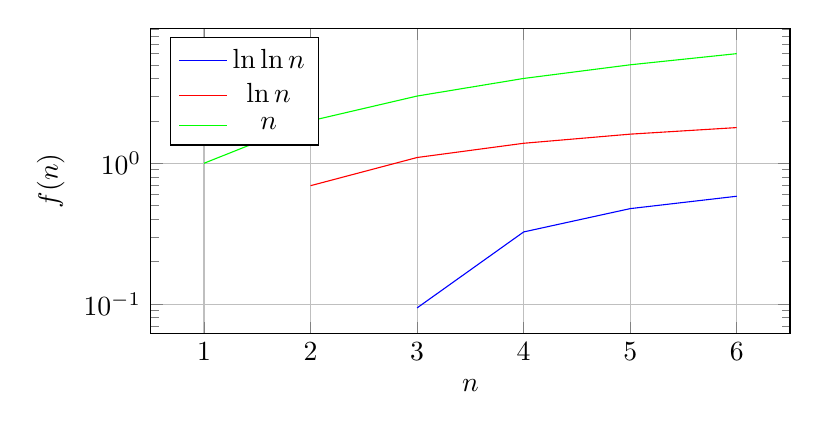
\begin{tikzpicture}
  \begin{axis}[
    width=0.8\textwidth, height=0.45\textwidth,
    xlabel={$n$}, ylabel={$f(n)$}, ymode=log,
    grid=major, legend pos=north west
  ]
    \addplot[blue,  mark=none] coordinates {(2,-0.3665) (3,0.0940) (4,0.3254) (5,0.4764) (6,0.5832)};
      \addlegendentry{$\ln\ln n$}
    \addplot[red,   mark=none] coordinates {(1,0) (2,0.6931) (3,1.0986) (4,1.3863) (5,1.6094) (6,1.7918)};
      \addlegendentry{$\ln n$}
    \addplot[green, mark=none] coordinates {(1,1) (2,2) (3,3) (4,4) (5,5) (6,6)};
      \addlegendentry{$n$}
  \end{axis}
\end{tikzpicture}
\end{center}

\subsection{Exercise 2}
For \(f,g,h\colon\mathbb N\to\mathbb R_{\ge0}\), prove:
\[
\begin{aligned}
1.\;&f\in O(f),\\
2.\;&O(c\,f)=O(f)\quad(\forall c>0),\\
3.\;&f(n)\le g(n)\text{ eventually}\implies O(f)\subseteq O(g),\\
4.\;&O(f)\subseteq O(g)\implies O(f+h)\subseteq O(g+h),\\
5.\;&h(n)>0\;\forall n,\;O(f)\subseteq O(g)\implies O(f\,h)\subseteq O(g\,h).
\end{aligned}
\]

\newpage

\textbf{Proof.}
\begin{enumerate}[label=\arabic*.]
  \item Since \(f(n)\le1\cdot f(n)\), we have \(f\in O(f)\).
  \item \(u\in O(c\,f)\) means \(u(n)\le C\,(c\,f(n))\), so \(u\in O(f)\).  Conversely the same argument shows \(O(f)\subseteq O(c\,f)\).  
  \item If \(f(n)\le g(n)\) for all large \(n\) and \(u\in O(f)\), then \(u(n)\le C\,f(n)\le C\,g(n)\), so \(u\in O(g)\).  
  \item If \(u\in O(f)\), then for large \(n\):
  \[
    u(n)+h(n)\;\le\;C\,f(n)+h(n)\;\le\;C\bigl(f(n)+h(n)\bigr),
  \]
  hence \(u+h\in O(f+h)\).  Since \(O(f)\subseteq O(g)\), also \(u+h\in O(g+h)\).  
  \item If \(u\in O(f)\) and \(h(n)>0\), then 
  \[
    u(n)\,h(n)\;\le\;C\,f(n)\,h(n)\;\le\;C\,C'\,g(n)\,h(n),
  \]
  showing \(u\,h\in O(g\,h)\).
\end{enumerate}

\paragraph{Constant-Factor Comparison}
\begin{figure}[h]
  \centering
  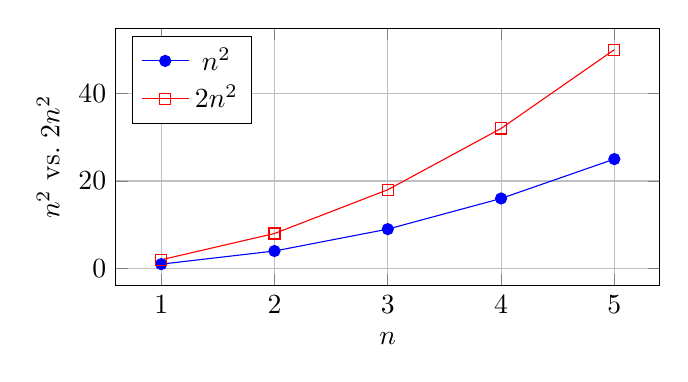
\begin{tikzpicture}
    \begin{axis}[
      width=0.7\textwidth, height=0.4\textwidth,
      xlabel={$n$}, ylabel={$n^2$ vs.\ $2n^2$},
      grid=major, legend pos=north west
    ]
      \addplot[blue,mark=*]   coordinates {(1,1) (2,4) (3,9) (4,16) (5,25)};
      \addlegendentry{$n^2$}
      \addplot[red,mark=square]coordinates {(1,2) (2,8) (3,18) (4,32) (5,50)};
      \addlegendentry{$2n^2$}
    \end{axis}
  \end{tikzpicture}
  \caption{Verifying \(O(c\,f)=O(f)\).}
\end{figure}

\subsection{Exercise 3}
Let \(i,j,k,n\in\mathbb N\).  Prove:
\[
\begin{aligned}
1.\;&j\le k\implies O(n^j)\subseteq O(n^k),\\
2.\;&j\le k\implies O(n^j+n^k)\subseteq O(n^k),\\
3.\;&O\Bigl(\sum_{m=0}^k a_m\,n^m\Bigr)=O(n^k),\\
4.\;&O(\log n)\subseteq O(n),\\
5.\;&O(n\log n)\subseteq O(n^2).
\end{aligned}
\]

\textbf{Proof.}
\begin{enumerate}[label=\arabic*.]
  \item If \(j\le k\), then \(n^j\le n^k\) for \(n\ge1\); hence any \(u\in O(n^j)\) satisfies \(u(n)\le C\,n^j\le C\,n^k\), so \(u\in O(n^k)\).
  \item For \(n\ge1\), \(n^j+n^k\le2n^k\).  If \(u\in O(n^j+n^k)\), then \(u(n)\le C(n^j+n^k)\le2C\,n^k\), so \(u\in O(n^k)\).
  \item \(\sum_{m=0}^k a_m\,n^m\le\bigl(\sum|a_m|\bigr)\,n^k\), hence \(O(\sum a_mn^m)=O(n^k)\).
  \item For \(n\ge2\), \(\log n\le n\), so \(O(\log n)\subseteq O(n)\).
  \item For \(n\ge2\), \(n\log n\le n^2\), so \(O(n\log n)\subseteq O(n^2)\).
\end{enumerate}

\subsection{Exercise 4}
Which relationships hold between:
\[
\begin{aligned}
1.\;&O(n)\text{ vs.\ }O(\sqrt n),\\
2.\;&O(n^2)\text{ vs.\ }O(2^n),\\
3.\;&O(\log n)\text{ vs.\ }O((\log n)^2),\\
4.\;&O(2^n)\text{ vs.\ }O(3^n),\\
5.\;&O(\log_2n)\text{ vs.\ }O(\log_3n).
\end{aligned}
\]
\textbf{Answer.}
\begin{enumerate}[label=\arabic*.]
  \item \(\sqrt n\le n\) for \(n\ge1\), so \(O(\sqrt n)\subsetneq O(n)\).
  \item \(n^2=o(2^n)\), hence \(O(n^2)\subsetneq O(2^n)\).
  \item Eventually \((\log n)^2\ge\log n\), so \(O(\log n)\subseteq O((\log n)^2)\).
  \item \(2^n\le3^n\), thus \(O(2^n)\subsetneq O(3^n)\).
  \item \(\log_2n=\tfrac{\log_3n}{\log_32}\), a constant factor, so \(O(\log_2n)=O(\log_3n)\).
\end{enumerate}

\subsection{Exercise 5}
Classic sorting comparisons:
\[
\text{bubble sort vs.\ insertion sort},\quad
\text{insertion sort vs.\ merge sort},\quad
\text{merge sort vs.\ quick sort}.
\]
\textbf{Discussion.}
\begin{itemize}
  \item \textbf{Bubble vs.\ Insertion:} Both worst-case \(O(n^2)\), but insertion sort is \(O(n)\) on nearly-sorted input.
  \item \textbf{Insertion vs.\ Merge:} Insertion sort worst-case \(O(n^2)\), merge sort always \(O(n\log n)\), so merge scales better.
  \item \textbf{Merge vs.\ Quick:} Merge sort is \(O(n\log n)\) always; quick sort is \(O(n\log n)\) average, \(O(n^2)\) worst, but faster in practice due to lower constants and in-place partitioning.
\end{itemize}

\section{Conclusion}
We’ve surveyed P vs.\ NP, NP-completeness via SAT, practiced ordering and relating functions by asymptotic growth, and applied these insights to sorting algorithms. The included plots illustrate constant-factor and growth-rate comparisons without overwhelming the presentation.

\begin{thebibliography}{9}
  \bibitem{italc}
    J.~E.~Hopcroft, R.~Motwani, and J.~D.~Ullman,
    \textit{Introduction to Automata, Languages, and Computation},
    Addison–Wesley, 3rd~ed., 2006.
\end{thebibliography}

\end{document}
